\documentclass[conference, anonymous]{IEEEtran}
\IEEEoverridecommandlockouts
% The preceding line is only needed to identify funding in the first footnote. If that is unneeded, please comment it out.
\usepackage{tikz}
\usetikzlibrary{shapes.geometric, arrows.meta, positioning}
\usepackage{cite}
\usepackage{amsmath,amssymb,amsfonts}
\usepackage{algorithmic}
\usepackage{graphicx}
\usepackage{textcomp}
\usepackage[most]{tcolorbox}
\usepackage{xcolor}
\usepackage{hyperref}
\usepackage{paralist}
\usepackage[most]{tcolorbox}
\usepackage{enumitem}
\usepackage{tabularx}
\usepackage{booktabs}
\usepackage{array}
\usepackage{float}      % optional (for exact positioning)
\usepackage{caption}    % optional (better captions)
\newcolumntype{Y}{>{\raggedright\arraybackslash}X}

\usepackage{geometry}
\geometry{margin=1in}


\definecolor{medgray}{gray}{0.85}
\def\BibTeX{{\rm B\kern-.05em{\sc i\kern-.025em b}\kern-.08em
    T\kern-.1667em\lower.7ex\hbox{E}\kern-.125emX}}

\newcommand{\nick}{\texttt{First, Do No Harm To the Data}}
\begin{document}

% \title{First, Do No Harm -- To the Data: A secure RAG and Dual-LLM Architecture for Medical Agents
\title{First, Do No Harm To the Data: RAG and Dual-LLM Architecture for Medical Agents
%\\
%{\footnotesize \textsuperscript{*}Note: Sub-titles are not captured in Xplore and
%should not be used}
%\thanks{Identify applicable funding agency here. If none, delete this.}
}

\author{\IEEEauthorblockN{Anonymous}
%\IEEEauthorblockA{\textit{dept. name of organization (of Aff.)} \\
%\textit{name of organization (of Aff.)}\\
%City, Country \\
%email address or ORCID}
% \and
% \IEEEauthorblockN{2\textsuperscript{nd} Given Name Surname}
% \IEEEauthorblockA{\textit{dept. name of organization (of Aff.)} \\
% \textit{name of organization (of Aff.)}\\
% City, Country \\
% email address or ORCID}
% \and
% \IEEEauthorblockN{3\textsuperscript{rd} Given Name Surname}
% \IEEEauthorblockA{\textit{dept. name of organization (of Aff.)} \\
% \textit{name of organization (of Aff.)}\\
% City, Country \\
% email address or ORCID}
% \and
% \IEEEauthorblockN{4\textsuperscript{th} Given Name Surname}
% \IEEEauthorblockA{\textit{dept. name of organization (of Aff.)} \\
% \textit{name of organization (of Aff.)}\\
% City, Country \\
% email address or ORCID}
% \and
% \IEEEauthorblockN{5\textsuperscript{th} Given Name Surname}
% \IEEEauthorblockA{\textit{dept. name of organization (of Aff.)} \\
% \textit{name of organization (of Aff.)}\\
% City, Country \\
% email address or ORCID}
% \and
% \IEEEauthorblockN{6\textsuperscript{th} Given Name Surname}
% \IEEEauthorblockA{\textit{dept. name of organization (of Aff.)} \\
% \textit{name of organization (of Aff.)}\\
% City, Country \\
% email address or ORCID}
}

\maketitle

\begin{abstract}


\end{abstract}

\begin{IEEEkeywords}
Clinical-Decision Making, Large Language Models, LLM-as-a-Judge
\end{IEEEkeywords}

\section{Introduction}
\label{sec:introduction}


% Clinical Decision-Making (CDM)~\cite{banning2008review} is about using the best information to make the right choice for patient care. It combines medical knowledge, doctor experience, and patient needs. This approach helps doctors pick treatments that work well and fit each patient.

% However, practicing CDM is becoming more difficult. Medical research is growing rapidly. There are many studies, reports, and articles to read~\cite{li2025large}. Searching through all this information, checking its quality, and applying it correctly takes alot of time and skills. Tools like the PICO (Patient, Intervention, Comparison, Outcome) framework help structure questions and filter studies~\cite{richardson1995well}, but the process is still slow and complex. Given the potential consequences of clinical error, this process must be both thorough and accurate.

% Large Language Models (LLMs) offer a promising way to support CDM~\cite{brugge2024large}. These models can understand and generate human-like text, helping with tasks like summarizing studies, answering clinical questions, and find important information quickly~\cite{tang2023evaluating}. Models like GPT-4~\cite{achiam2023gpt} have shown strong performance on medical exams and other healthcare tasks, showing they can assist doctors in making better decisions.

% Despite their promise, general-purpose LLMs face key challenges in clinical use. They often lack the deep medical knowledge required to handle complex or highly specialized clinical tasks~\cite{jung2025large}. Also, these models can generate "hallucinations" -- answers that sound confident but are factually wrong or unsafe~\cite{zhang2025siren}. This is especially risky in healthcare settings. To address this, researchers have turned to multi-agent LLM frameworks~\cite{yao2025survey}. These systems mimic how real doctors work together when making clinical decisions. Some examples are RareAgents~\cite{chen2024rareagents}, MDAgents~\cite{kim2024mdagents}, AMSC~\cite{wang2024beyond}, AMIE~\cite{tu2024towards}, Dr-House~\cite{yang2024drhouse}, MEDAIDE~\cite{wei2024medaide}, MEDIQ~\cite{li2024mediq}, Exploring the Inquiry~\cite{liu2025exploring}. For example, \textit{Exploring the Inquiry}~\cite{liu2025exploring} simulates and AI hospital workflow that covers the full process from patient consultation to diagnosis, while MEDIQ~\cite{li2024mediq} supports multi-round doctor-patient interactions to iteratively collect missing information and refine diagnosis. 

% Inspired by how real clinical teams collaborate, MDAgents~\cite{kim2024mdagents} introduces an adaptive decision-making framework that uses LLMs to emulate hierarchical diagnostic workflows -- from individual doctor to collaborative  clinical teams. MDAgents works in four steps \begin{inparaenum}[\it (i)] \item assessing the complexity of a case \item  Recruiting appropriate agents based on that medical complexity; \item Performing collaborative analysis and synthesis, and \item producing a final response. \end{inparaenum} 

% However, a key limitation of MDAgents lies in its lack of a second-level validation step. Once an answer is made -- whether by a solo doctor or clinical team -- it is treated as the final decision. There is no mechanism to review, critique, or improve the response. This absence of feedback is problematic, especially in medicine, where LLM-generated responses must be carefully evaluated for accuracy, completeness, and safety before they can be trusted in clinical settings.

% Another big challenge in using LLMs for CDM is keeping patient information private. Medical reports, case report, and trial data, contain sensitive personal information. Sharing this data with large models can risk exposing private information. This raises serious concerns about data privacy. 
% There are privacy-preserving techniques to protect privacy, such as using cryptographic methods~\cite{khan2023learning, khan2023love, khan2023more, khan2024make, khan2024wildest} and data anonymization~\cite{wimmer2016multi}. These help keep patient information safe. While this is an important research direction, our current work does not focus on privacy issues.

% In our proposed approach, we build upon the MDAgents framework by adopting a multi-agent LLM architecture for CDM. The process begins with the system evaluating the complexity of the medical query. Based on clinical criteria, the case is categorized as basic, intermediate and advanced. Depending on this classification, the framework activates either a single Primary Care Physician (PCP) for basic queries,  or Multi-disciplinary Team (MDT) or Integrated Care Team (ICT) for intermediate and advanced medical queries.

% After collaborative reasoning and synthesis, the final response generated by the agents is submitted to a specialized evaluation component called LLM-as-a-Judge. This judging model takes both the original medical query and the generated answer as input. It then assigns an evaluation score based on several key attributes: the inclusion of essential medical information, accuracy of the answer, completeness, safety, and clarity. This evaluation step ensures that the final response is not only clinically sound but also aligned with best practices in CDM.

Modern medical AI systems increasingly rely on Retrieval-Augmented Generation (RAG), where an AI model retrieves information from external sources such as research databases, health forums, and clinical websites before generating an answer. While this approach improves knowledge coverage, it also introduces serious safety and security risks. The core problem is that current RAG-based medical agents do not control how retrieved information influences reasoning and decision- making. As a result, low-quality, misleading or even malicious content can shape medical conclusions, recommendations, or tool actions. 

In particular, these systems treat all retrieved text as neutral context, without distinguishing between high-trust sources like peer-reviewed research and low-trust sources like anonymous online forums. Furthermore, even when planning and reasoning components are isolated, there is typically no mechanism that controls how retrieved  data flows through the system or how it affects sensitive actions such as treatment recommendation or external tool calls. Therefore, there is a clear need for a more secure architecture that can track the origin of retrieved information and enforce strict policies on how that information is allowed to influence medical reasoning and actions.


To understand the problem more clearly, imagine a medical AI assistant that receives a patient's question. The system retrieves information from different sources, such as academic research articles, clinical guidelines, and online patient discussion boards. All of this retrieved text is then given to the language model, which uses it to generate a diagnosis or treatment suggestion. 

At first glance this seems powerful and helpful. However, the problem begin with the assumption that all retrieved information can be treated equally. In reality, a peer/reviewed clinical study and an anonymous forum comment do not carry the same level of reliability. Yet once they are placed into the model's context window, the system does not inherently understand these differences in trust. As a result, incorrect information may influence clinical reasoning just as much as validated medical evidence.

The situation becomes even more concerning when consider prompt injection. Suppose someone posts malicious or misleading instructions inside a public health forum. If the RAG system retrieves that content, the language model may unintentionally incorporate those instructions into its reasoning process. Even if the overall task planning remains correct, the data being used to make decisions has already been compromised. In other words the control flow maybe safe, but the data flow is not.

This distinction between control flow and data flow is crucial. Protecting control flow means ensuring that the system follows the correct sequence of steps. Protecting data flow means ensuring that the information used within those steps is trustworthy and allowed to influence certain outcomes. In medical contexts, unsafe data flow can lead to incorrect diagnosis, inappropriate treatment suggestions, or unauthorized access to sensitive tools such as prescription system or medical records.

Another important aspect of the problem is action sensitivity. Medical AI agents may not only generate text but also interact with tools. They might write notes ito electronic health records, generte prescriptions or send reports. If untrusted retrieved information influences these actions, the consequences are much more serious than simply generating a wrong sentence. The system could produce harmful clinical decisions or violate privacy constraints.

Current defense strategies, such as isolating planning models from data/proessing models, improve security but do not fully solve this issue. They focus mainly on preventing malicious instructions from alerting the system's plan. However, they do not prevent malicious or low-quality data from shaping the content of decisions within that plan. In other words, they protect how the system acts, but not what information it uses to decide.

Therefore, the fundamental research challenge is to design a medical RAG architecture that does not merely retrieve and generate, but also understands where each piece of information comes from and enforce rules about how it can be used. The system must be able to differentiate between trusted and untrusted sources, track how retried data influences reasoning, and block or restrict actions when that influence violates safety policies. 

In summary, the problem is not simply about improving accuracy. It is about ensuring that medical AI systems remain safe, robust, and trustworthy when interacting with diverse and potentially unreliable external knowledge sources. Without mechanism to control data flow and influence, RAG based medical agents remain vulnerable to subtle but potentially dangerous failures.

\paragraph{Contribution}

The main contributions of this paper are: \newline


\section{Preliminaries}
\label{sec:preliminaries}

Retrieval-Augmented Generation (RAG) systems combine a retrieval module (which fetches relevant documents or knowledge) with a generative language model (LLM). This enables the LLM to ground its responses in external, possibly up-to-date, or domain-specific information. \cite{zhou2025privacyaware}

\section{Related Work}
\label{sec:relatedwork}

Digital healthcare is changing how patients receive care through technologies like wearable devices and AI tools. These allow doctors to monitor patients remotely, create personalized treatments, and predict health issues \cite{jeddi2020remote}. ML tracks how diseases progress, while language models understand medical notes to support better decisions. Together, these tools make healthcare more efficient, accurate, and accessible~\cite{shen2024large}. Dual LLM system splits an AI assistant into a privileged LLM (talks to trusted sources and uses tools) and a quarantined LLM (used anytime on untrusted content and expected to go rogue anytime) that can safely use tools and private data while mitigating prompt injection attacks \cite{willison2023dual}.

% LLMs are very good in generating human-like text and understand complex language. In healthcare, LLMs are used for tasks such as answering medical exam questions~\cite{lievin2024can}, conducting biomedical research~\cite{thapa2023chatgpt}, and assisting diagnosis~\cite{mcduff2025towards}. They have also been tested with generating medical report summaries, clinical decision support, and even virtual health assistants. By saving doctors time, LLMs contribute to more efficient and patient-friendly care~\cite{tripathi2024efficient}. 

% Interactive healthcare conversational systems are important for providing patients with accurate and relevant information. Datasets and benchmarks like MedQA~\cite{jin2021disease} and MedMCQA~\cite{pal2022medmcqa} have helped improve question-answering systems in medicine. These systems use large datasets to fine-tune LLMs, making their responses more relevant and patient-centered. 

% Recent research shows that using multiple LLMs together(multi-agent systems), can outperform single models~\cite{li2023camel, chen2024agentverse, wu2024autogen}. In these systems, each agent has a specific role, and they break down complex tasks into smaller parts~\cite{li2023camel, wu2024autogen}. Another approach involves, agents debating each other's answer to arrive at better solutions, often improving accuracy and reasoning~\cite{du2023improving, wang2025learning, liu2025truth}. Other forms of collaboration include group voting~\cite{DBLP:conf/iclr/0002WSLCNCZ23}, expert discussions~\cite{DBLP:conf/acl/ChenSB24}, or even negotiation~\cite{bianchi2024well}. While these approaches are promising, they usually work with fixed settings that may not work well across all tasks~\cite{liu2024dynamic}. In some setups, this can lower performance or use up extra resources on easy tasks.

% To address this, MDAgents~\cite{kim2024mdagents} propose a dynamic approach that adjusts the collaboration strategy based on the complexity of task. It classifies clinical tasks as low, moderate or high complexity using CDM techniques. This is useful in CDM, where teamwork, flexibility, and reasoning are essential. However, while MDAgents use different collaboration strategies, they lack an explicit mechanism for evaluating and assessing the quality of generated response, which is critical in healthcare. 

% To fill this gap, we introduce an LLM-as-a-Judge component -- a clinically informed evaluation system that reviews agent outputs for accuracy and quality. Different types of LLM-as-a-judge exist~\cite{zheng2023judging}, some compare two answers and choose the better one; other score a single answer directly; and some use reference answers to guide grading. This judging approach has several benefits such as allowing faster and larger-scale evaluation and provides explanation along with scores, making its assessment transparent. RAGAS~\cite{es2024ragas} -- LLM-as-a-Judge framework, has gained widespread adoption for the evaluation of Question Answering (QA) systems. It receives the generated answer, the correct answer, and sometimes the question. Then, using clear scoring rules and carefully designed prompts, the judge scores the response. %Importantly, in our deployed LLM-as-a-Judge component, if the judge finds an answer of low quality, it flags the case for a human expert to review. This human-in-the-loop setup ensures that final answers are reliable and safe for clinical use.

\section{\nick}
\label{ssec:methodology}

\subsection{Agent Roles}
\label{subsec: agent-roles}

\section{Methodology}

\begin{figure*}[t]
    \centering
    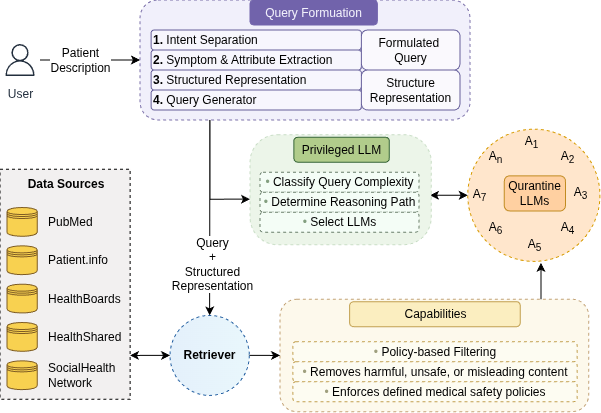
\includegraphics[width=\textwidth]{CamelMedAgents-RAG-workflow-updated.png}
    \caption{Proposed CaMel Multi-Agent RAG Framework for Medical Query Processing. 
    The system consists of a Query Formulation module, structured representation generation, 
    RAG retrieval from multiple medical data sources, privileged LLM reasoning, 
    moderation, quarantine LLMs, and policy-based safety enforcement.}
    \label{fig:camel_rag_workflow}
\end{figure*}


\subsection{Query Formulation}
\label{subsec: query-formulation}
The first stage of our methodology focuses on transforming raw user input into a clinically precise and retrieval-ready query. Since medical questions from users are often informal, emotional, or loosely structured, directly using them for retrieval can reduce accuracy and introduce ambiguity. Therefore, we design a multi-step query formulation pipeline that gradullay refines the input while preserving its meaning. 
\begin{enumerate}
    \item \textbf{Intent Separation (LLM):} We begin with intent separation. When a uer describes their symptoms, they often include conversational elements such as filler words, persnal concerns, or emotional expressions. For example, a user might say, "...................". While this conveys important context, it also contain lexical noise that can negatively affect retrieval performance. In this step an LLM carefully rewrites the input into clinically focused language  without changing the underlying meaning. The goal is not to reinterpret or diagnose, but simple to clarify and normalize the expression. As a result, the system produces a cleaner an medically oriented version of the query that retains semantic fidelity while reducing ambiguity.
    
    \item \textbf{Symptom \& Attribute Extraction (LLM):} Once the query has been clarified, the next step is symptom and attribute extraction. At this stage, the LLM identifies explicitly metioned clinical entities such as symptoms, duration, severity,a ge, gender, and any othe relevant modifiers. Instead of working wit free-form text, the system now begins converting the information into structured medical variabless. for example ............. This transformation is important because structured variablesare more stable and suitable for downsteam reasoning and retrieval. It also reduces the risk that later stages of the system rely on vague or unstructured representations.  
    
    \item \textbf{Structured Representation (Deterministic):} After extraction, the pipeline moves to structured representation, which is fully deterministic. Unlike previous steps, this stage does not involve further LLM reasoning. Instead, the extracted information is mapped into a canonical schema with predefined fields. The purpose of this step is threefold. First, it clearly separates clinical presentation from meta information such as emotional tone or background context. Second, it provides a stable and standarized structure that can be consistently used for retrieval, evaluation, and auditing. Third, by removing generative flexibiltiy at this stage, it prevents hallucinated details from propagating further into the system. In other words, once the information is structured, it becomes fixed and transparent. 
    
    \item \textbf{Query Generator (Deterministic):} With structure data in place, the system proceed to query generator., which is also deterministic. Here, the goal is to convert the structured clinical variables into retrieval-optimized search queries without introducing new semantic variation. This ensures that the meaning remains consistent with the original user intent. Two type of wueries are generated in parallel. The first is a dense retrieval query, which takes the normalized symptoms and modifiers and reformulates  them into a natural clinical sentence. This version is designed for embeding-based vector search. The second is a sparse retrieval query, which convert the same structured variables into a boolean-style keyword query suitable for traditional lexical search methods. By keeping this stage deterministic, we ensure that no unintended reinterpretation occurs.
    
    \item \textbf{Dense + Sparse Retrieval Query:} Finally, the system performs hybrid retrieval using both dense and sparse queries. Medical queries often suffer from vocabulary mismatch. Patients may use everyday language, whereas scientific literature uses technical terminology. Dense retrieval helps bridge this gap by captuing semantic similarity through vector embeddings. At the same time, sparse retrieval method such as BM25 remain highly effective for exact keyword matching, especially for specific medical terms. Therfore, the dense reformulated query is embedded and used for vector search, while the sparse boolena query is used for key-word-based retrieval. The result from both methods are then merged or re-ranked to produce a final candidate set of documents.

    By combining these steps in a structured and sequestial manner, the query formulation stage ensures  that retrieval begins with a clean, clinically grounded, and semantically stable representation of the user's concern. This careful preparation not only improves retrieval quality but also strengthens the overall robustness and safety of the system.
\end{enumerate}

\subsection{RAG over External Medical Sources}
\label{subsec: rag-externalsources}

Once the query has been carefully formulated and structured, the system moves to the retrieval stage. At this point, the input is no longer informal user text. Instead, it is a clean, clinically organized representation that is optimized for searching medical knowledge sources. This makes the retrieval process more accurate and controlled. 

TO begin with, the system sends the generated dense and sparse queries to external data sources. These sources may include: Pubmed, patientinfo, healthboards, healthsahred, and socialhealth networks. Because the query has already been cleaned and normalized, the search process is more focused and less likely to retrieve irrelevant content.

First, the dense retrieval query is used for semantic search. The system convert this query into a vector embedding and compares it with pre-indexed document embeddings stored in a vector database. This allows the system to find documents that are conceptually similar,even if they do not use the exact same wording. For example, if a patient describe ".........." the system can still retrieve documents discussing "........." because the embedding captures meaning rather than just keywords. This step helps reduce the gap between everyday language and medical terminology.

At the same time, the sparse retrieval query is applied using traditional keyword-based search methods such as BM25. This approach focuses on exact term matching and is especially useful when the query includes specific medical terms, drug names, or well-defined conditions. While dense retrieval captures meaning, sparse retrieval ensures precision. By running both searches in parallel, the system benefits from the strength of each method.

After both retrieval processes are complete, the results are combined. The system may merge the document list or re-rank them based on relevance score. At this stage, the goal is to select a balanced and high-quality set of candidate documents. The system also applies the filtering rules, such as removing duplicate entries, excluding extremely low-quality scores, and ensuring diversity across trusted domains.

Once the relevant documents are selected, the system does not immediately pass them to reasoning model. Instead, each document is processed carefully. The content is segmented into manageable chunks so that specific passages can be analyzed independently. In addition, metadata, such as source type , publication origin and trust level is attached to each chunk. This step is important because it prepares the documents for the next stage, where capability policies will control how the information is used.
At this point, the retrieval stage is complete. The system has transformed a structured clinical query into a curated set of relevant medical evidence gathered from multiple sources. More importantly, the retrieved content is not treated as neutral text.  It is organized, labeled, and prepared for controlled reasoning. This ensures that the next stages of pipeline can operate on well-structures and traceable information rather than raw and potentially unreliable data.

In this way, the retrieval stage act as a bridge between query formulation and safe reasoning. It ensures that the system gathers meaningful and relevant medical knowledge while maintaining organization and transparency, which are essential for building a secure and reliable medical AI system.

\subsection{Capabilities}
\label{subsec: capabilities}

After retrieving information from external medical sources, the first step in ensuring safe and reliable reasoning is to assign capabilities to every piece of information. Capabilities are essentially metadata that describe the origin, trust level and allowed usage of data. They act as "tags" that travel with the information throughout the system, guiding how it can be stored, merged, or used in reasoning.

For example, a peer reviewed article from PubMed may be labeled as high-trust scientific evidence, while posts from patient forums or social health networks might be tagged as low-trust anecdotal information. If a document contains sensitive patient  information, it receives additional restrictions specifying who is allowed to access or act upon it.  Capabilities are also granular. Each value or variable derived from a document -- such as symptom, lab results, or treatment recommendation - carries its own tag. These tags track the source of the data, any intermediate transformations, and the allowed readers or tools that can access it. For instance, a lab result extracted from a patient forum post might be restricted from being directly used in medical recommendation, whereas the same type of information from a clinical guideline could be fully usable.

By attaching capabilities at the earliest stage, the system preserve a clear record of data provenance and reliability. In short capabilities act as a foundation for our system's safe reasoning. they make it possible to merge and process heterogeneous medical sources responsibly, track the origin and quality of information, and enforce fine-grained rules on what can and cannot be used in generating responses. 

\subsection{Knowledge Consolidation and Query-Specific Databases}
\label{subsec: query-specificd-databases}

Once capabilities have been assigned to all retrieved documents -- capturing their source, trust level, and any restrictions, the next step is to consolidate and organize the information in  meaningful way. Capabilities serve as a guide during this process, ensuring that only appropriate and reliable data is merged while preserving provenance and restrictions. Instead of treating each retrieval cycle as temporary, the system merges the selected documents and builds a structured knowledge base around the specific type of query. In other words, for every clinical query, the system gradually creates its own focused database. To explain this more clearly, lets look at the following cases:

For the Acne label, user discuss persistent breakouts, rosacea-like redness, concerns about isotretinion side effects, and treatment failures. Even though the wording is different, the core theme is similar: acne management and treatment concerns. Guided by capabilities system retrieves relevant medical guidelines and research, then merges them into an acne-specific database. Over time, this database grows to include evidence on isotretinoin, topical treatments, rosacea overlap, and mental health considerations.

For the appendicitis label, users describe ruptured appendix complications, cheonic diarrhea after surgery, wound infections, and fear of delayed rupture. these posts share a common theme of appendicitis and post-surgical outcomes. The system uses capabilities to ensure that reliable, medical sound information is selected, consolidating about appendectomy recovery, complications, bowel changes, and warning signs into an appendicitis-specific database, which is updated as similar queries appear.

Similarly, for the cancer label, users worry about small, dark skin spots and whether they might be dangerous. Using capabilities to prioritize trusted sources like dermatology guidelines, the system gather information about mole assessment and melanoma signs. The information is then organized into a skin-cancer-related database that supports future queries about suspicious lesions.

After retrieval, all relevant documents are connected to that theme are then combined and stored together. Over time, this creates a query-specific knowledge repository. As new queries are processed in the future, the system does not start from the scratch, Instead it updates the corresponding database by adding newly retrieved relevant documents removing outdated or low quality entries, and refining the stored content. This means the knowledge base becomes richer and more precise with use. The more frequently a particular query type appears, the more complete and robust its associated database becomes.  

This structure creates smaller, focused databases instead of one large and messy collection of information. Each database is linked to a specific query or medical category. For example, there can be one database for acne-related questions, another for appendicitis cases, and another for cancer concerns and so on.  This design has clear benefits. First, it makes the system faster and more efficient, because when a new query comes in, it can first look at the already built database for that category instead of searching everything from the scratch.. Second it keeps answers more consistent, since similar cases rely on the same growing pool of information. Third it improves transparency, because the system can track which database contributed to a particular response.

\subsection{Security Policies}
\label{subsec: security-policies}

While capabilities describe what the data is, security policies define what can be done with it. In our system, policies enforce rules such as:
\begin{itemize}
    \item High-trust evidence can be used for reasoning and answering queries, while low-trust anecdotal content may only provide context.
    \item Sensitive or personally identifiable information cannot be used without explicit user permission. 
    \item Conflicting information is resolved by prioritizing high-trust sources, with uncertainties clearly flagged.
    \item Database updates must preserve capabilities, ensuring that provenance and restrictions are maintained even after consolidation.
\end{itemize}

These policies are expressed programmatically, allowing the system to enforce fine-grained rules. They prevent low-trust or restricted data from influencing outputs in unsafe ways, while allowing high-quality information to guide reasoning.

\subsection{Interpreter}
\label{subsec: interpreter}

\begin{figure}[h]
\centering
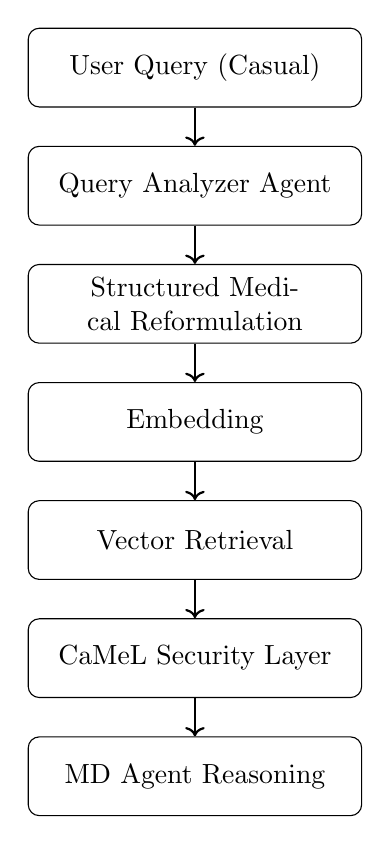
\begin{tikzpicture}[
    node distance=1.5cm,
    box/.style={rectangle, draw, rounded corners, text width=4cm, align=center, minimum height=1cm},
    arrow/.style={->, thick}
]

\node (A) [box] {User Query (Casual)};
\node (B) [box, below of=A] {Query Analyzer Agent};
\node (C) [box, below of=B] {Structured Medical Reformulation};
\node (D) [box, below of=C] {Embedding};
\node (E) [box, below of=D] {Vector Retrieval};
\node (F) [box, below of=E] {CaMeL Security Layer};
\node (G) [box, below of=F] {MD Agent Reasoning};

\draw [arrow] (A) -- (B);
\draw [arrow] (B) -- (C);
\draw [arrow] (C) -- (D);
\draw [arrow] (D) -- (E);
\draw [arrow] (E) -- (F);
\draw [arrow] (F) -- (G);

\end{tikzpicture}
\caption{CaMeL Methodology Architecture}
\end{figure}



\begin{figure}[h]
\centering
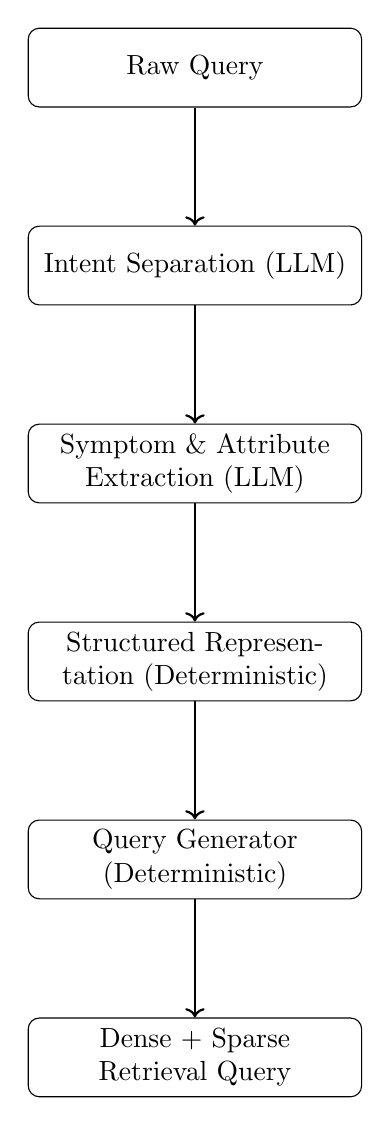
\begin{tikzpicture}[
    node distance=1.5cm,
    box/.style={
        rectangle, 
        draw=black, 
        rounded corners, 
        text width=4cm, 
        align=center, 
        minimum height=1cm
    },
    arrow/.style={->, thick}
]

\node (A) [box] {Raw Query};
\node (B) [box, below=of A] {Intent Separation (LLM)};
\node (C) [box, below=of B] {Symptom \& Attribute Extraction (LLM)};
\node (D) [box, below=of C] {Structured Representation (Deterministic)};
\node (E) [box, below=of D] {Query Generator (Deterministic)};
\node (F) [box, below=of E] {Dense + Sparse Retrieval Query};

\draw [arrow] (A) -- (B);
\draw [arrow] (B) -- (C);
\draw [arrow] (C) -- (D);
\draw [arrow] (D) -- (E);
\draw [arrow] (E) -- (F);

\end{tikzpicture}
\caption{Query Formulation Pipeline}
\end{figure}

\section{Dataset}
For the Queries dataset, we are using the \cite{7889534} dataset that contains patient descriptions and the classified disease of the description. This dataset contains \textbf{11104} patient descriptions.

\section{Data Curation}
As we only have queries dataset available but not relevant data against the queries, that is the requirement of RAG.
So, we are creating the dataset by scraping the following sources:
\begin{enumerate}
    \item PubMed
    \item Patient Info
    \item HealthBoards
    \item HealthShared
    \item SocialHealthNetwork
\end{enumerate}


\section{Medical Parameters Extraction}

In medical question answering systems, patient queries are typically expressed in informal, unstructured language containing a mixture of symptoms, contextual details, and non-clinical expressions. Directly using such input in retrieval pipelines introduces semantic ambiguity, vocabulary mismatch, and uncontrolled propagation of noisy signals into downstream reasoning \cite{demner2009nlp,trec2017}. This is particularly critical in medical RAG systems, where unstructured inputs can lead to unsafe data flow and reduced reliability.

To address this, we design a \textit{Medical Parameters Extraction} module that transforms raw patient queries into a structured clinical representation. This representation serves as a controlled intermediate layer that standardizes clinical signals before they are used in query formulation and data curation. By enforcing structure at this stage, the system ensures that downstream components operate on well-defined and auditable variables rather than free-form text.

Formally, given a patient query $q$, the objective is to extract a structured representation $S$ consisting of clinically relevant attributes:
[
S = {S_{\text{sym}}, S_{\text{temp}}, S_{\text{ctx}}, S_{\text{int}}}
]
where $S_{\text{sym}}$ denotes symptoms, $S_{\text{temp}}$ temporal information, $S_{\text{ctx}}$ patient context, and $S_{\text{int}}$ clinical interpretation.

\subsubsection{A. Extraction Architecture}

The extraction process is implemented as a multi-stage pipeline, where each stage focuses on a specific clinical signal. Instead of performing all extraction tasks within a single model invocation, the problem is decomposed into smaller, well-defined subtasks. This design reduces signal interference and improves extraction fidelity, particularly for symptom identification, which forms the primary driver of retrieval in symptom-centric medical queries.

Each stage produces a structured output constrained by a predefined schema. The outputs are sequentially aggregated to construct the final representation $S$. This modular design enables better control over data transformation and supports traceability of extracted attributes, which is essential for enforcing safe data flow in later stages of the system.

\subsubsection{B. Symptom Extraction}

The first stage focuses on identifying symptoms explicitly described in the query. Symptoms are treated as primary clinical signals, as medical retrieval is predominantly symptom-driven rather than diagnosis-driven.

A key challenge in this step is linguistic variability. Patients often describe symptoms using non-clinical expressions, which differ from standardized medical terminology. To address this, the system performs normalization by mapping informal expressions to clinically recognized terms, improving alignment with medical literature and retrieval systems \cite{devlin2019bert}.

Each symptom is represented as a structured tuple:
[
(\text{name}, \text{normalized_name}, \text{location}, \text{severity})
]
where attributes are included only if explicitly mentioned. No implicit inference is performed at this stage.

\subsubsection{C. Temporal Information Extraction}

The second stage extracts temporal characteristics associated with the reported symptoms. Temporal information plays a critical role in clinical decision-making and diagnosis \cite{rajkomar2018}.

This stage identifies attributes such as duration, onset type, and frequency, and normalizes them into standardized representations. When multiple symptoms exhibit different temporal patterns, the system constructs a symptom-level temporal mapping to preserve these distinctions.

To maintain factual integrity, temporal attributes are extracted strictly from explicit statements in the query. Missing information is not inferred, ensuring that downstream reasoning is based only on observed data.

\subsubsection{D. Patient Context Extraction}

The third stage extracts patient-specific contextual factors that may influence clinical interpretation. These include age, gender, pregnancy status, and comorbidities.

Contextual variables act as modifiers that refine the interpretation of symptoms and guide both retrieval and reasoning. Comorbidities are restricted to explicitly stated pre-existing conditions and are carefully distinguished from current symptoms or speculative diagnoses.

\subsubsection{E. Clinical Interpretation}

The final stage captures higher-level semantic intent and potential risk signals present in the query. This stage performs two tasks: intent classification and red-flag detection.

Intent is categorized into predefined classes such as diagnosis, treatment, reassurance, emergency, or prognosis. In parallel, the system detects clinically significant risk patterns (red flags) based on established indicators of potentially severe conditions. When such patterns are identified, they are explicitly flagged to enable stricter downstream safety policies.

\subsubsection{F. Structured Representation and Integration}

The outputs of all stages are aggregated into a unified structured representation $S$, which is validated against a predefined schema to ensure consistency and completeness.

This structured representation enables deterministic and semantically stable query generation, guides data curation and scraping strategies, and supports safe data flow by ensuring that all extracted variables are explicit and traceable. By converting unstructured patient input into a standardized clinical format, this module establishes a reliable interface between user queries and the RAG pipeline.



\section{Scraping Strategy}
To scrape data accurately, we follow the following steps:

\subsection{Data Analysis}
Understand the dataset:
\begin{enumerate}
    \item Count Descriptions per label
    \item Group the diseases into categories
\end{enumerate}

To scrape the relevant data per description, we need to extract the information important from a medical point of view. This includes:
\begin{enumerate}
    \item Symptoms
    \item Anatomical Location
    \item Onset
    \item Frequency
    \item Triggers
    \item Age
    \item Gender
    \item Pregnancy Status
    \item Comorbidities
    \item Clinical Intent
    \item Clinical Flags
    \item Duration
    \item Severity

\end{enumerate}

\section{Performance Analysis}
\label{sec: performance-analysis}

\subsection{Experimental Setup}
\begin{enumerate}
    \item OS Ubuntu 24.04.3 LTS
    \item Processor AMD Ryzen™ 7 6800H 
    \item RAM 16 GB
    \item LLM GPT 4o mini
\end{enumerate}

\subsection{Experimental Results}

\section{Discussion:}
\textbf{11th December'2025} \newline 
Based on the experimental results, we can dive into the implementation of guardrails and policies for detecting injection and performing countermeasures in the following directions:
\begin{enumerate}
    \item User, can be malicious [low priority]
    \item Dataset / Data Center, retrieved data from RAG [high priority]
    \item Both user and dataset [low priority]
\end{enumerate}
Q: How to implement this on RAG? \newline
A: Rough idea
\begin{enumerate}
    \item detecting malicious instruction from retrieve chunks
\end{enumerate}


\section{Conclusion and Future Direction}
\label{sec: conclusion}



\bibliographystyle{IEEEtran}
\bibliography{references}


\section{Privacy-Aware RAG: Secure and Isolated Knowledge Retrieval - Summary ChatGPT}

\end{document}
\section{Performance Analysis}
\label{sec: performance-analysis}

\subsection{Datasets}
\label{subsec:datasets}

\paragraph{PubMedQA} It is a biomedical question-answering (QA) dataset collected from PubMed abstracts~\cite{jin2019pubmedqa}. The task of PubMedQA is to answer research questions with \textit{yes/no/maybe} using the corresponding abstracts. It has 1K expert annotated, 61.2k unlabeled and 211.3k artificially generated QA instances. Each PubMedQA instance is composed of a 1) question which is either an existing research article title or derived from one, 2) a context which is the corresponding abstract without its conclusion, 3) a long answer which is the conclusion of the abstract and, presumably, answer the research question, and 4) a \textit{yes/no/maybe} answer which summarizes the conclusion. 


\section{Conclusion}
\label{sec:conclusion}

% \section*{Acknowledgment}



\end{document}
